\documentclass[a4paper, fleqn]{article}
\usepackage{chemfig}
\usepackage{mhchem}
\usepackage{xcolor}
\usepackage{amsmath}
\usepackage{tikz}
\usepackage{chemfig}
\usepackage{amssymb}
\usepackage{hyperref}
\usepackage{chemfig}
\usepackage[
  left=1cm,
  right=1cm,
  top=2cm,
  bottom=2cm,
]{geometry}

\def\cc{ç}
\def\Cc{Ç}

\title{Organische Chemie}
\date{8. Februar 2024}
\author{ACHTUNG\\Dieses Dokument ersetzt KEINE Literatur und oder Pr\"asenz in den Vorlesungen.\\Alle Informationen eurer Dozenten k\"onnen in einer Klausur gefordert werden.\\Es ist die eigene Aufgabe, diese zu lesen bzw. zu besuchen und sich darum zu bem\"uhen sie zu verstehen.\\Au\ss erdem garantiert das Dokument keine komplette Lehr-/Studiumsgrundlage.}

\begin{document}
\tableofcontents
\newpage
\maketitle
\hrule

\section{Organische Chemie}
\subsection{Organische Molek\"ule}
\subsubsection{Darstellung von organischen Molek\"ulen}
\begin{itemize}
  \item Gr\"o\ss tm\"gliche Anzahl an Oktetten
  \item Ladungen gem\"a\ss der Elektronegativit\"at 
  \item M\"oglichst geringe Ladungstrennung
  \item[$\rightarrow$] Oktett wichtiger als Ladungstrennung
\end{itemize}

\subsubsection{Benennung der organischen Molek\"ule}
\begin{itemize}
  \item[] Grundprinzipien: \begin{itemize}
    \item Stammname f\"ur das Ger\"ust
    \item Substituenten
    \item Positionsziffern f\"ur die Position der Substituenten
  \end{itemize}
\end{itemize}

\subsubsection{Regeln der Nomenklatur}
\begin{itemize}
  \item l\"angste Kette gibt den Stammnamen (\dots , Pentan, Hexan, Heptan, \dots)
  \item Substituentennamen enden auf '-yl' (Methyl, Ethyl, Propyl, \dots)
  \item Nummerierung der Kette so, dass sich m\"oglichst kleine Zahlen f\"ur die Positionen der Substituenten ergeben
  \item Namen zusammensetzen: \begin{itemize}
    \item Stammname am Ende 
    \item Substituenten davor in alphabetischer Reihenfolge
    \item Positionsziffern mit Bindestrichen vor Substituenten (1,3,5-[Name des Substituenten] \dots)
    \item Wenn ein Substituent mehrfach vorkommt: Pr\"afixe (Di-, Tri-, Tetra-, \dots)
  \end{itemize}
\end{itemize}

\subsection{Acidit\"at}
\subsubsection*{Wie stark sind Molek\"ule als Br\o nsted-S\"auren}
Der Trend im Periodensystem der Elemente zeigt, je h\"oher die Ordnungszahl, umso h\"oher liegt die Acidit\"at. Dasselbe gilt f\"ur Elemente die in einer 'tieferen' Periode stehen.\\
Resonanzstabilisierung (mehr m\"ogliche mesomere Grenzstrukturen) der konjugierten Base.\\
Je stabiler die entstehende Base, desto st\"arker die vorliegende S\"aure.\\

\subsubsection{Hybridisierung}
Je h\"oher die $\mathrm{sp^n}$-Hybridisierung, desto schw\"acher die jeweilige S\"aure. 

\subsubsection{Induktiver Effekt}
Seitenketten und einzelne Substituenten wirken durch ihre Elektronegativit\"at im Vergleich zu den anderen Elementen und Verbindungen einen 'dr\"uckend/schiebenden' oder 'ziehenden' Effekt auf die Elektronendichte aus.\\
Dadurch wird die Stabilit\"at und somit die Reaktionsf\"ahigkeit der Verbindungen beeinflusst.\\
Instabiler $\rightarrow$ reagiert besser, niedrigerer $p\mathrm{K_s}$-Wert, st\"arkere S\"aure.

\subsubsection{Effekt von Solvatisierung}
Acidit\"at von Essigs\"aure in Wasser: $p\mathrm{K_s} = 4,8$, im Vakuum: $p\mathrm{K_s}\approx 130$\\
Somit ist die Acidit\"at auch von Umgebung und Gemisch abh\"angig.

\subsection{Basizit\"at}
\subsubsection{Hybridisierung}
Es gilt das Reverse wie bei der Acidi\"at.\\
Je h\"oher die $\mathrm{sp^n}$-Hybridisierung, desto st\"arker die jeweilige S\"aure. 

\subsection{Alkane}
\begin{itemize}
  \item ges\"attigte Kohlenwasserstoffe
  \item allgemeine Summenformel \ce{C_nH_{2n+2}}
  \item Cycloatome z.B.: Cyclohexan, allgemeine Summenformel: \ce{C_nH_{2n}}
  \item homologe Rate der Alkane ergibt sich formal durch Einschub der Methylengruppen\\
      \begin{center}
        \begin{tabular}{c c}
          \hline
          \ce{H3C-H} & Methan\\
          \ce{H3C-CH2-H} & Ethan\\
          \ce{H3C-CH2-CH2-H} & Propan\\
          \vdots & \vdots\\
          \hline
        \end{tabular}
      \end{center}
\end{itemize}

\subsubsection{Isomere}
Isomere haben die gleiche Summenformel, jedoch unterchiedliche Strukturen.\\
Stellt man alle Kohlenstoffatome einfach in eine Reihe, so nennt sich das, zum Beispiel bei Heptan, $n$-Heptan.

\subsubsection{Reaktion der Alkane}
Reaktionsm\"oglichkeiten:\\
heterolytischer (ungleicher) Bindungsbruch, ein Atom erh\"alt mehr Elektronen als das jeweils andere, an dessen Verbindung gebrochen wird.\\
$\rightarrow$ Ionenbildung.\\
homolytischer (gleicher) Bindungsbruch, beide Atome erhalten dieselbe Anzahl an Elektronen.\\
$\rightarrow$ Radikalbildung.\\\\
Chlorierung von Methan, Mechanismus:\\\\
Kettenstart\\
\ce{Cl-Cl -> Cl\cdot $+$ \cdot Cl}\\\\
Kettenfortpflanzung\\
\ce{Cl \cdot $+$ H-CH3 -> Cl-H + Cl-CH3}\\
\ce{Cl-Cl + \cdot CH3 -> Cl\cdot $+$ Cl-CH3}\\\\
Kettenabbruch\\
\ce{Cl\cdot $+$ \cdot Cl -> Cl-Cl}\\
\ce{Cl\cdot $+$ \cdot CH3 -> Cl-CH3}\\
\ce{H3C\cdot $+$ \cdot CH3 -> H3C-CH3}\\\\
Es k\"onnen auch h\"here chlorierte Produkte entstehen, da diese Reaktiver sind als das Edukt.\\
Radikale k\"onnen durch Hyperkonjugation stabilisiert werden. (Wechselwirkung eines unbesetzten und besetzten Orbitals, die benachbart sind)

\subsubsection{Reaktivit\"at \& Selektivit\"at}
Beispiel: Bromierung von Propan.\\
Brom pr\"aferiert hierbei die Position mit der Positionsziffer 2 (am mittleren Kohlenstoff) ($>$99\%).\\
Die Bindung an das Ende der Kohlenstoffkette ist mit $<$0,5\% sehr unwahrscheinlich.

\subsection{Alkene}
Kohlenwasserstoffe mit Doppelbindung.\\
Bei einer Doppelbindung sind die $\pi$-Orbitale beteiligt.\\
die Nomenklatur sieht somit auch vor, dass die Position der Doppelbindung durch die Positionsziffer angegeben wird.\\
Priorit\"aten f\"ur die Substituenten an den C-Atomen der Doppelbindung festlegen.\\
je h\"oher die Ordnungszahl des gebundenen Elements, umso h\"oher die Priorit\"at.\\
Wenn die zwei Substituenten h\"ohere Priorit\"aten auf der gleichen Seite sind (Z)/cis auf entgegengesetzte (E)/trans

\subsubsection{Elektrophile Addition an Alkenen}
\ce{CH2=CH + HCl -> H3C-CH2Cl}\\
\ce{CH2=CH2 + H2O ->[{Katalysator, S\"aure}] H3C-CH2-OH}\\
\ce{CH2=CH2 + Br2 -> Br-CH2-CH2-Br}\\

Mechanismus der Addition, zweistufig.\\
\ce{H2C=CH-CH3 + HBr <-> H3C-CH^+-CH3 + H2C^+-CH2-CH3}\\
Das erste Produkt ist hierbei ein sekund\"ares Carbeniumion, das mittlere Kohlenstoff ist positiv geladen. Das zweite Produkt ist ein prim\"ares Carbeniumion, hierbei ist der erste (linke) Kohlenstoff positiv geladen.\\
REGEL VON MARKORNIKOV: Bei der Addition von \ce{HX} geht der Wasserstoff an de Kohlenstoff, der bereits mehr Wasserstoffatome tr\"agt.\\
Ein Terti\"ares Carbeniumion ist stabiler als ein sekund\"ares, welches stabiler als ein prim\"ares ist, da diese durch die Hyperkonjugation beeinfluss werden kann.\\\\

Addition von \ce{Br2} an Alkenen:\\
\ce{CH2=CH2 + Br-Br -> Br-CH2-CH2 + Br^- <-> \chemfig{\ce{CH2}?[a]-\ce{CH2}(-[3]\ce{Br}?[a])} + Br^- -> Br-CH2-CH2-Br}\\
Redox-Reaktion m\"oglich.\\
\ce{H2C=CH2 + Br-Br -> H2C-CH2^+ + Br^--Br}\\

Bei der Bromierung von Propen setzt das Brom unwahrscheinlicher an das Ende der Kohlenstoffkette (1-Brompropan), sondern setzt sich eher als Seitenkette an. (Hauptprodukt 2-Brompropan)\\

\subsection{Alkine}
Kohlenwassertstoffe mit Dreifachbindungen.

\subsubsection{Nomenklatur}
Endung: -in; Pentin, Hexin, Heptin. Hierbei wird auch wieder die Positionsziffer der Dreifachbindungen angegeben.

\subsubsection{Chemische Eigenschaften/Reaktionen}
Acidit\"at von Alkinen\\
\ce{R-\chemfig{C~C}\vert^- + CO2 -> R-\chemfig{C~C'}-COO^-}\\
Elektrophile Addition von HCl\\\\
\ce{CH2=CH2 + HCl -> H2C=CHCl} (Vinylchlorid)\\
Hydrierung\\
\ce{R_a-\chemfig{C~C}-R_b + H2 -> R_aHC=CHR_b}

\subsection{Halogenalkane}
\subsubsection{Nomenklatur}
Behandlung von Halogensubstituenten analog zu Alkylsubstituenten. (Siehe 1.1.3)\\
\subsubsection{Besondere Eigenschaften}
\begin{itemize}
  \item Bilden eigene Phasen
  \item Schmelzpunkt liegt niedriger als bei dem jeweiligen reinen Kohlenwasserstoff.
  \item Dichte h\"oher als bei Kohlenwasserstoffen
  \item Reaktionstr\"age
\end{itemize}
\subsubsection{Verwendung}
K\"altemittel, Treibstoff, Narkosemittel
\subsubsection{Darstellung (Herstellung) von Halogenalkanen}
\begin{itemize}
  \item Radikale Substitution bei Alkanen
  \item Alektrophile Addition von Halogen-Wasserstoff Verbindungen an Alkenen
  \item Addition von \ce{Br2}
\end{itemize}
\subsubsection{Reaktionen}
nukleophile Substitution\\
\ce{NaSH + CH3Br -> CH3-SH + NaBr}\\
\subsubsection*{Unterschiede der \ce{SN^1} und \ce{SN^2} Reaktion}
Nach der Faustregel reagieren prim\"are Halogenide reagieren nach \ce{SN^2}, sekund\"are nach \ce{SN^1 \& SN^2}, terti\"are nach \ce{SN^1}\\
\subsubsection*{Reaktionen von und zu Halogenalkanen}
Bei der Eliminierung wird das jeweilige Halogen aus der Verbindung 'eliminiert/entfernt', wobei z.B. bei einem Cyclohexen mit einem Brom als Substituenten eine Doppelbindung zur\"uckbleibt.\\
Bei der Addition von \ce{Br2} and Cyclohexen wird die Doppelbindung aufgebrochen um beide Bromatome als Substituenten an dieses gebunden werden.

\subsubsection{Isomere}
Definition unter 1.4.1.\\
Konstitutionsisomere haben eine unterschiedliche Abfolge der Bindungen\\
Enantiomere sind wie Bild und Spiegelbild (Siehe Chiralit\"at f\"r besseres Verst\"andnis)\\
Diastereomere verhalten sich NICHT wie Spiegelbilder zueinandern.

\subsubsection*{Benennung von Stereogenen Zentren/Stereoisomeren}
Betrachtung des stereogenen Zentrums\\
\begin{itemize}
  \item Ordnen der Substituenten nach ihrer Priorit\"t\\H\"ohere Ordnungszahl $\rightarrow$ H\"ohere Priorit\"at\\Doppel-\&Dreifachbindungen werden wie zwei Bindungen behandelt.
  \item Betrachtung so, dass Substituenten niedriger Priorit\"at nach hinten zeigen.
  \item Wenn \"ubrige substituenten im Uhrzeigersinn (R)\\ Gegen den Uhrzeigersinn (S)
\end{itemize}

\subsubsection*{Eigenschaften von chiralen Substituenten}
\begin{itemize}
  \item Sind in einer achiralen Umgebung gleich, bis auf die Drehung von linear polarisiertem Licht (Genaueres wird in der VL zur PC und den Laboren des AP und der PC erl\"autert)
  \item Drehung des polarisierten Lichts ist entgegengesetzt der Richtung durch die beiden Enantiomere (+) oder (-) Richtung
  \item Es liegt keine einfache Korrelation zwichen (R)/(s) und (+)/(-)
  \item Anderes (historisches) System zur Benennung der stereochemischen Konfiguration D/L (Sollte von Kohlenwasserstoffen bekannt sein, falls nicht D-Glucose\&L-Glucose nachschlagen)
  \item Nach Fischer (Fischerprojektion, bekannt aus selbigen vorherigen Materialien, falls nicht, Kohlenwasserstoffe nachschlagen oder Aminos\"auren)
\end{itemize}

\subsection{Chemie der Ether}
\subsubsection{Reaktionen}
williamische Ethersynthese\\
Benzylisierung\\
Etherspaltung\\
\ce{CH3-CH2-O-CH2-CH3 ->[{HBr}] CH3-CH2-OH + Br-CH2-CH3} (Heterolytische Spaltung des \ce{HBr})\\

\subsection{Aromatische Verbindungen}
Monozyklische, planare, vollst\"andig konjugiert, delokalisiertes $\pi$-Elektronensystem.\\
Am Bekanntesten ist hierbei Benzol mit seinen mesomeren Grenzstrukturen (Zeichnen mit Doppelbindungen nicht mit dem Kreis im Kohlenwasserstoff).\\
$\rightarrow$ Cyclohexan $\neq$ Benzol (DOPPELBINDUNGEN!)
\subsubsection{Elektrophile aromatische Substitution}
Experiment aus der Vorlesung genauer betrachten.\\
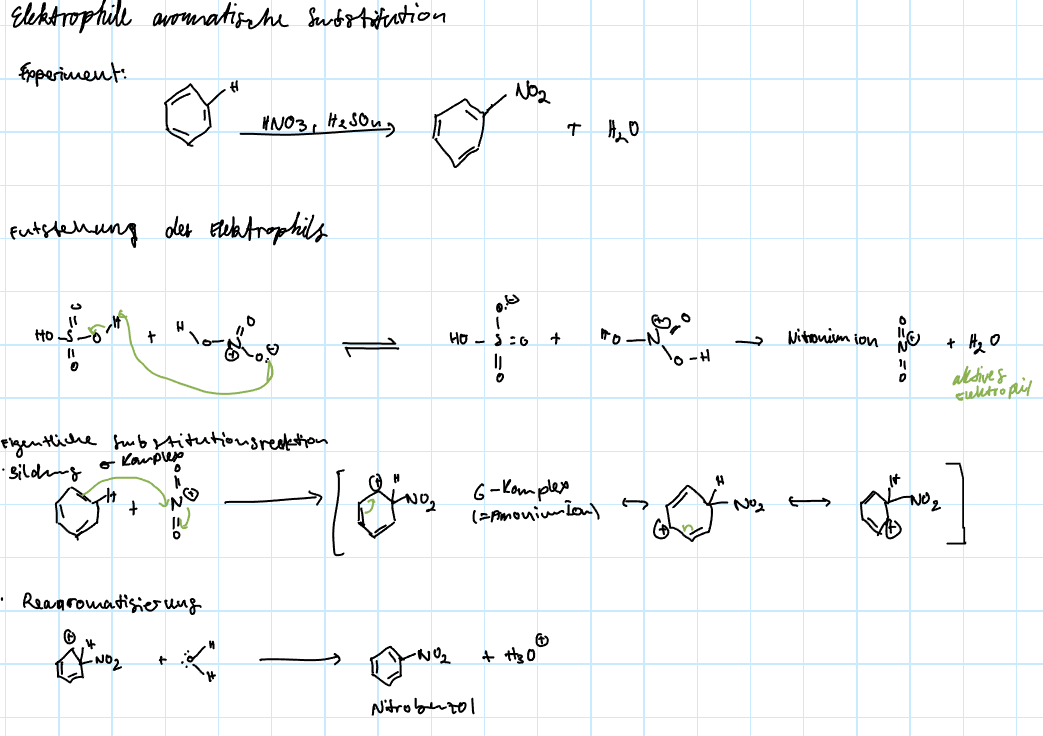
\includegraphics[width=0.9\pdfpagewidth]{egrs.PNG}\\
\begin{center}
  Abb.1: Zeichnung/Aufschrieb von Zeyneb Zahide \Cc etintas
\end{center}
\subsubsection{Chlorierung von Benzol}
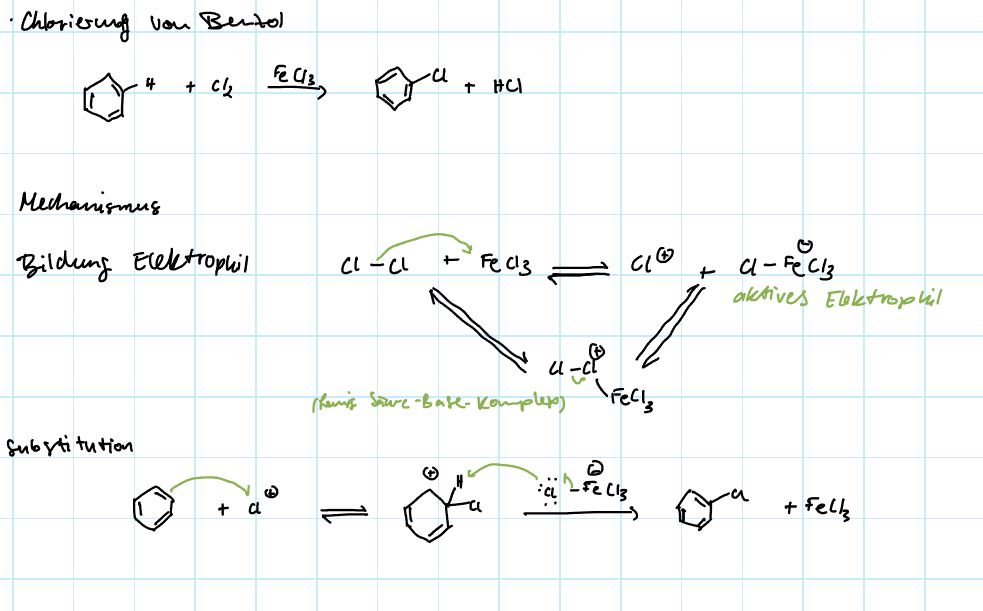
\includegraphics[width=0.9\pdfpagewidth]{knogh.PNG}
\begin{center}
  Abb.2: Zeichnung/Aufschrieb von Zeyneb Zahide \Cc etintas
\end{center}
\subsubsection{Friedl-Craft-Alkylierung}
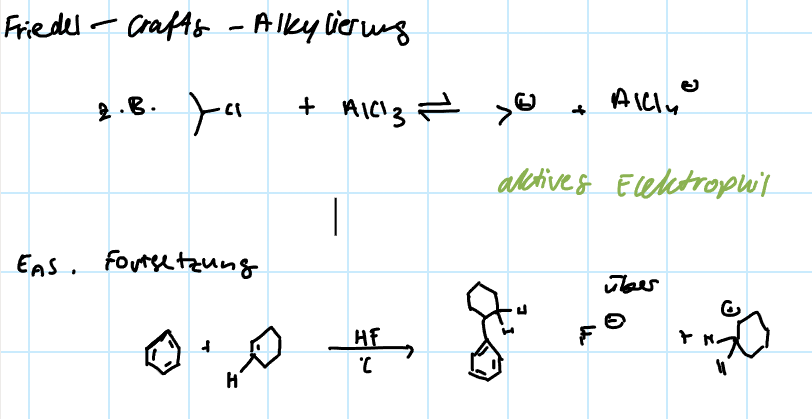
\includegraphics[width=0.9\pdfpagewidth]{hjrty.PNG}
\begin{center}
  Abb.3: Zeichnung/Aufschrieb von Zeyneb Zahide \Cc etintas
\end{center}
\subsubsection{Friedl-Craft-Acylierung}
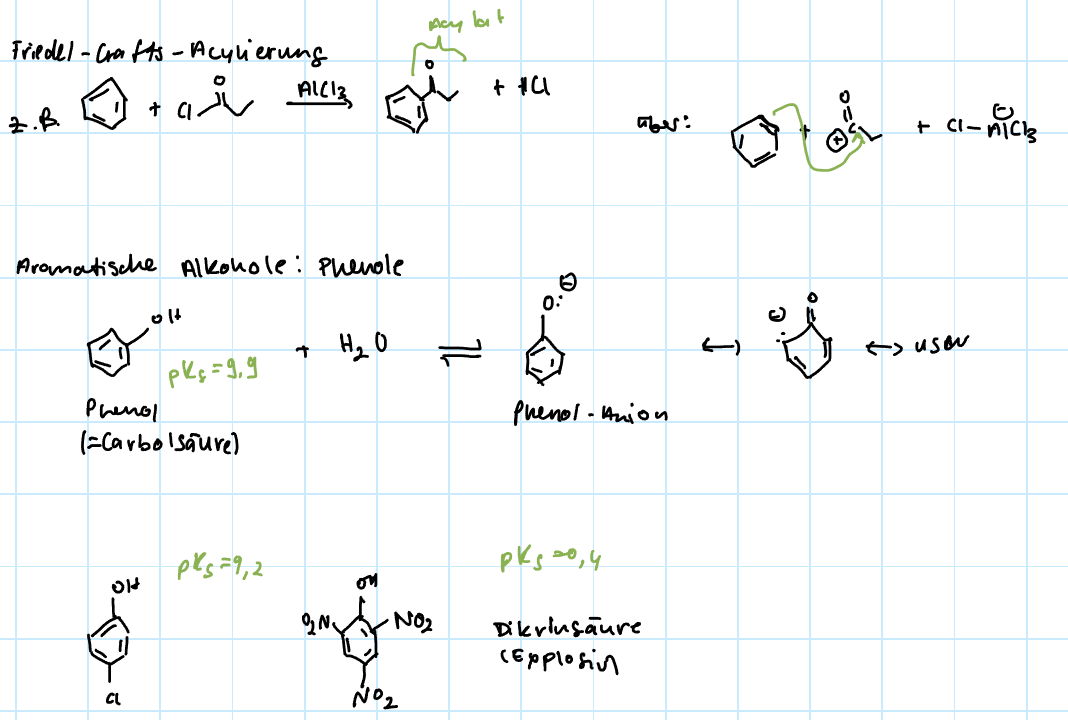
\includegraphics[width=0.9\pdfpagewidth]{klinka.PNG}
\begin{center}
  Abb.4: Zeichnung/Aufschrieb von Zeyneb Zahide \Cc etintas
\end{center}
\subsection{Carbonylverbindungen}
enthalten die Carbonylgruppe\\
\ce{R_a-CO-R_b} Ketone\\
\ce{H-CO-R} Aldehyde\\
\subsubsection{Nomenklatur}
Aldehyde haben die Endung '-al'\\
Ketone haben die Endung '-on'\\
Bei der Benennung haben Ketone und Aldehyde eine h\"ohere Priorit\"at.
\subsubsection{Grundlagen der Reaktivit\"at von Carboxylverbindungen}
\subsubsection{Friedl-Craft-Aklylierung}
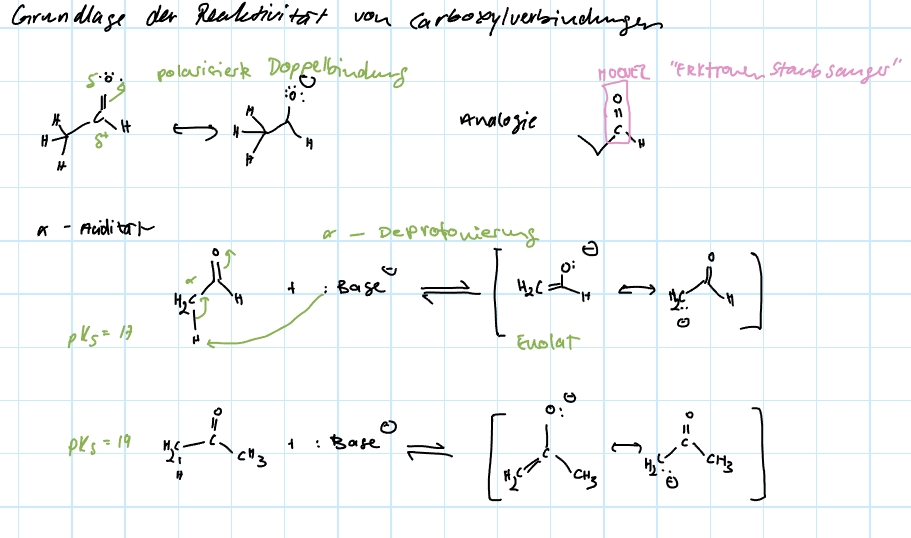
\includegraphics[width=0.9\pdfpagewidth]{knogg.PNG}
\begin{center}
  Abb.5: Zeichnung/Aufschrieb von Zeyneb Zahide \Cc etintas
\end{center}
\subsubsection{Keto-Enol-Tautomerie \& S\"aurekatalysierte Tautomerisierung}
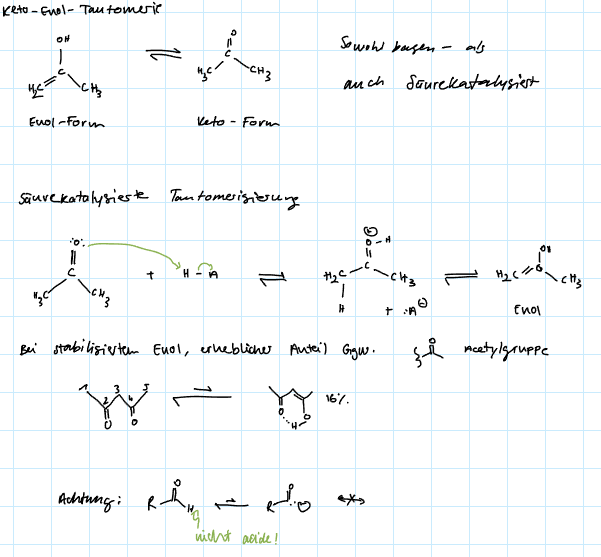
\includegraphics[width=0.9\pdfpagewidth]{ninjaball.PNG}
\begin{center}
  Abb.6: Zeichnung/Aufschrieb von Zeyneb Zahide \Cc etintas
\end{center}
\end{document}